\documentclass[10pt,conference,letterpaper]{IEEEtran}
\special{papersize=8.5in,11in}
\usepackage{latexsym}
\usepackage{amsfonts}
\usepackage{amsmath}
\usepackage{amssymb}
\usepackage{color}
\usepackage{epsfig}
\usepackage{xspace}
\usepackage{graphicx,epstopdf}
\usepackage{stfloats}
%\usepackage{times}
\usepackage{subfigure}
\usepackage{cite}
\usepackage{balance}
\usepackage{amsmath, bm}
\usepackage[english]{babel}
\usepackage{array}
\usepackage{multirow}

\pdfpagewidth=8.5in
\pdfpageheight=11in

\newcommand{\eat}[1]{}
\newcommand{\sttab}{\rule{0pt}{8pt}\\[-3ex]}
\newcounter{ccc}
\newcommand{\bcc}{\setcounter{ccc}{1}\theccc.}
\newcommand{\icc}{\addtocounter{ccc}{1}\theccc.}
\newcommand{\myhrule}{\rule[.5pt]{\hsize}{.5pt}}
\newcommand{\mat}[2]{{\begin{tabbing}\hspace{#1}\=\+\kill #2\end{tabbing}}}
\newcommand{\stitle}[1]{\vspace{0.5ex}\noindent{\bf #1}}
\newcommand{\etitle}[1]{\vspace{0.5ex}\noindent{\em \underline{#1}}}
\newcommand{\marked}[1]{\textcolor{red}{#1}}
\newcommand{\markedb}[1]{\textcolor{blue}{#1}}
\newcommand{\subsubtitle}[1]{\vspace{0.5ex}\noindent\underline{{\bf #1}}}

%\newcommand{\stab}{\rule{0pt}{8pt}\\[-1.6ex]}
%\newcommand{\sttab}{\rule{0pt}{8pt}\\[-2ex]}
\newcommand{\sstab}{\rule{0pt}{8pt}\\[-2ex]}
\newcommand{\bi}{\begin{itemize}}
\newcommand{\ei}{\end{itemize}}

\newcommand{\ie}{\emph{i.e.,}\xspace}
\newcommand{\eg}{\emph{e.g.,}\xspace}
\newcommand{\wrt}{\emph{w.r.t.}\xspace}
\newcommand{\aka}{\emph{a.k.a.}\xspace}
\newcommand{\kw}[1]{{\ensuremath {\mathsf{#1}}}\xspace}

\newcommand{\oursystem}{\kw{Athena}}
\newcommand{\sarank}{\kw{SARank}}

\begin{document}


\title{A Ranking and Profiling-based Scholarly Data Analysis System}
%\title{\oursystem: A Ranking-based Scholarly Analysis System}
\title{A Ranking-based Scholarly Analysis System}

% author names and affiliations
% use a multiple column layout for up to three different
% affiliations
\eat{
\author{\IEEEauthorblockN{Michael Shell}
\IEEEauthorblockA{School of Electrical and\\Computer Engineering\\
Georgia Institute of Technology\\
Atlanta, Georgia 30332--0250\\
Email: http://www.michaelshell.org/contact.html}
\and
\IEEEauthorblockN{Homer Simpson}
\IEEEauthorblockA{Twentieth Century Fox\\
Springfield, USA\\
Email: homer@thesimpsons.com}
\and
\IEEEauthorblockN{James Kirk\\ and Montgomery Scott}
\IEEEauthorblockA{Starfleet Academy\\
San Francisco, California 96678--2391\\
Telephone: (800) 555--1212\\
Fax: (888) 555--1212}}
}%%% eat original format author

\author{\IEEEauthorblockN{Junfeng Liu, Shuai Ma, Renjun Hu and Jinpeng Huai}
\IEEEauthorblockA{SKLSDE Lab, Beihang University, Beijing, China}
\IEEEauthorblockA{Beijing Advanced Innovation Center for Big Data and Brain Computing, Beijing, China}
\{liujunfeng, mashuai, hurenjun, huaijp\}@buaa.edu.cn}
%liujunfeng, mashuai, hurenjun, huaijp

\maketitle


\begin{abstract}
Scholarly analysis systems greatly enhance scientific knowledge discovery and propagation.
%
Recently, a number of scholarly analysis systems have been developed. However, these systems barely support ranking heterogenous scholarly entities under different metrics and, hence, fail to answer questions such as which authors/venues/affiliations are recently the most relevant/important in the queried field of study. In addition, existing systems adopt RDBMS or distributed file systems as their storage solutions, whereas the linked feature of scholarly data is largely ignored.
%
To this end, in this paper, we design and develop \oursystem, a novel scholarly analysis system. Our \oursystem supports heterogeneous scholarly entity rankings and is equipped with both traditional relevance- and citation-based and more recent importance-based ranking metrics. Moreover, \oursystem utilizes a popular graph database Neo4j as the storage solution. The linked structures are directly leveraged to facilitate the efficiency of graph query processing.
%Based on the above, we have built an online service for scholarly analysis.
We demonstrate two use cases in scholarly entity ranking and profiling and the advantage of Neo4j-based storage compared with RDBMS.
\end{abstract}
% Up to now, some systems have been developed with a tremendous amount of scholarly data and providing a range of functions to query keywords. However, these systems barely support different types ranking or various entities ranking (\itshape e.g.,\upshape venues, affiliation and authors) when researchers tend to get better knowledge about the keywords. In the paper, we design and develop a novel ranking system for scholarly data analysis that uses graph engine to efficiently manage the heterogeneous, evolving and dynamic natures of structured scholarly data and integrates different types ranking and various entities ranking based on SARank.  bring great convenience in querying scholarly data and discovering knowledge.


\IEEEpeerreviewmaketitle

\section{Introduction}
\label{sec-intro}


% Contributions: (1) heterogeneous entity ranking, (2) graph database for scholarly data management, (3) demonstration
%% Why heterogeneous entity ranking:
%% Why graph database:


% background
%Scholarly analysis systems greatly enhance scientific knowledge discovery and propagation.
The continuous advancements in science and engineering have contributed to an ever-expanding body of scientific literature.
As a result, it is becoming more and more challenging for people to follow the related research progress timely.
With this in the background, scholarly analysis systems are studied and developed to enhance scientific knowledge discovery and propagation. Basically, these systems enable to {\em rank} related scholarly entities (\eg articles, authors) given a query and, better, {\em profile} those retrieved entities.

%Scientific publications accelerate the dissemination of scientific discoveries all around the world. However, it is becoming more challenging to manage scientific advancement nowadays, due to the huge volume of scientific articles published.
%Consequently, ranking systems play a more important role for efficient scholarly data analysis than ever before.


% Search Engine | supporting entities | ranking metric | url
% Google Scholar | Article & Author | hybrid (full text, venue, author, how often and recently has been cited), mainly based on citation number
% Microsoft Academic | Article & Author | hybrid (how often and to which a publication is cited)
% Semantic Scholar | Article & Author | citation velocity
% CiteSeerX: | Article & Author | citation analysis: PageRank and coauthorship network
% Aminer: Article & author | Relevance, Year, #Citation
% AceMap: Article & author | authors, venues of key words, based on the numbers | https://acemap.info


%difference with existing systems
In the academic and industry, a number of scholarly analysis systems have been developed. Given a query of a specific research topic,  Google Scholar {\scriptsize (https://scholar.google.com/)}, Semantic Scholar {\scriptsize (https://www.semanticscholar.org/)} and CiteSeerX~\cite{li2006citeseerx} only ranks scholarly articles while AMiner~\cite{tang2008arnetminer} further gives rankings for authors. Also, the supported ranking metrics in these systems are either simple (\eg time and relevance) or biased to older articles (\eg citation-based).
%
On the other hand, Microsoft Academic {\scriptsize (https://academic.microsoft.com/)} and AceMap~\cite{tan2016acemap} do rank heterogenous entities, \ie articles, authors, venues and affiliations. However, AceMap simply ranks those entities based on the numbers of associated articles relevant to the query, and Microsoft Academic does by inferring query intent (based on the data from Bing).
%
To conclude, these systems may face challenges in ranking heterogeneous entities simultaneously with certain comprehensive metric.

%Given a query, these systems rank scholarly articles according to publish time, relevance or other citation-based metrics. %For instance, Google Scholar
%However, a majority of them do not support ranking other heterogenous entities, \eg authors, venues and affiliations, in a specific field of study, expect that , and it is unclear how Microsoft Academic does \marked{focus on user intension Bing vs. we give a comprehensive recommendation based on relevance and importance}. Moreover, the established ranking metrics are either simple (\eg time and relevance) or biased to older articles (\eg citation-based). Hence, they are insufficient to identify influential scholarly entities in an early stage.
%


%ranks articles mainly based on the number of citation, while Semantic Scholar proposes to use the citation velocity, which is a weighted average number of article citations in the last three years. On the other hand, CiteSeerX exploits weighted PageRank on the citation networks to determine the ranks of articles~\cite{sun2007popularity}.
%Besides, they also allow to retrieve and rank authors given author names.


%\marked{the reason for using Neo4j}
Besides, storage is another key factor for the success of scholarly analysis systems, due to the large volume of data (\eg MAG~\cite{sinha2015overview} contains 126 and 529 million articles and citations, respectively) and the complex relationships between entities.
%Traditional RDBMS are used by CiteSeerx, AMiner and Semantic Scholar to manage scholarly data. On the other hand, Acemap and Microsoft Academic exploit distributed file systems.
Existing systems mainly exploit RDBMS as their storage solutions.
%
We observe that scholarly entities are inherently linked. Existing systems all ignore such linked feature, and may be inferior in answering complex scholarly queries~\cite{BigGraphSearch}. For instance, complex joins in RDBMS will become the bottleneck when {\em finding the top-k articles of an author}.

%To this end, we propose to utilize a popular graph database Neo4j to store and manage the large-scale, heterogeneous and linked scholarly data in \oursystem.

%may face challenges for efficient and high-concurrent query processing when the computing resources are limited
%compared with structure-aware storage solutions


\begin{table}[t!]
\label{tab-function}
\begin{center}
\caption{Functions implemented in \oursystem and other systems}
\vspace{-1ex}
\begin{scriptsize}
\begin{tabular}{|c|c c c c|c c c c|}
\hline
\multirow{2}{*}{\bf Systems}   &  \multicolumn{4}{c|}{\bf Topic-dependent ranking}     & \multicolumn{4}{c|}{\bf Visual profiling}  \\
&  {\bf AR} & {\bf AU} & {\bf VE} & {\bf AF}  & {\bf AR} & {\bf AU} & {\bf VE} & {\bf AF} \\ \hline \hline
MS Academic & $\surd$ & $\surd$ & $\surd$ & $\surd$ & \marked{$\times$} & \marked{$\times$} & \marked{$\times$} & \marked{$\times$} \\
Google Scholar & $\surd$ & \marked{$\times$} & \marked{$\times$} & \marked{$\times$} & \marked{$\times$} & \marked{$\times$} & \marked{$\times$} & \marked{$\times$} \\
Semantic Scholar & $\surd$ & \marked{$\times$} & \marked{$\times$} & \marked{$\times$} & \marked{$\times$} & $\surd$ & \marked{$\times$} & \marked{$\times$} \\
CiteSeerX & $\surd$ & \marked{$\times$} & \marked{$\times$} & \marked{$\times$} &\marked{$\times$} & \marked{$\times$} & \marked{$\times$} & \marked{$\times$} \\
AMiner & $\surd$ & $\surd$ & \marked{$\times$} & \marked{$\times$} &  \marked{$\times$} & $\surd$ &  \marked{$\times$} &  \marked{$\times$}\\
AceMap & $\surd$ & $\surd$ & $\surd$ & $\surd$ & \marked{$\times$} & $\surd$ & $\surd$ & $\surd$ \\
\oursystem & $\surd$ & $\surd$ & $\surd$ & $\surd$ & $\surd$ & $\surd$ & $\surd$ & $\surd$ \\ \hline
\end{tabular} \\ \vspace{.5ex}
AR, AU, VE and AF stand for article, author, venue and affiliation, respectively.
\end{scriptsize}
\vspace{-4ex}
\end{center}
\end{table}

%(in honor of her wisdom and justice)
\stitle{Contributions}.
To this end, in this paper, we design and develop \oursystem, a novel scholarly analysis system to facilitate deep understanding of scholarly data. The functions of \oursystem and other systems are summarized in Table~I.

\noindent (1) \oursystem supports ranking four types of scholarly entities under five ranking metrics. Besides the traditional ones, we further equip \oursystem with a more advanced importance-ensemble metric that has proven effective for identifying important articles in an early stage~\cite{ma2018query}.

\noindent (2) \oursystem also supports profiling scholarly entities, \eg author profiling with research interest evolution and affiliation profiling with author and field of study visualization.

\noindent  (3) \oursystem utilizes graph database Neo4j {\scriptsize (https://neo4j.com)} for storage. To do this, we carefully design a Neo4j schema and represent the data as a huge property graph. We also incorporate Lucene index to enhance query efficiency.

\noindent (4) We have built a prototype system for \oursystem. We demonstrate two use cases in scholarly entity ranking and profiling and the advantage of storage with Neo4j compared with RDBMS. We will provide online service via Web and API.

%Our system implements a range of functions including: (i) article ranking by different ranking models given query keywords, (ii) heterogeneous entity rankings based on importance and (iii) detailed description and statistics of articles, authors, venues and affiliations.

%easily and efficiently search academic information by keywords; (ii) rank various scholarly entities (\itshape i.e., \upshape article, author, affiliation and venue) by different ranking type (\itshape i.e., \upshape SARank, relevance rank, citation and year); (ii) check home pages of affiliation, author, venue  \itshape etc.\upshape ; (iv) find detailed information about an article.

\stitle{Organization}.
The rest of this paper is organized as follows. Section \ref{sec-model} introduces the ranking model of \oursystem. The system overview is presented in Section \ref{sec-system}, followed by the demonstration in Section~\ref{sec-demo} and conclusions in Section \ref{sec-conc}.

\section{Scholarly Search and Ranking Model}
\label{sec-model}





In this section, we first introduce scholarly search, and then present the ranking model that lays its core foundation.


\subsection{Scholarly Search}
Our \oursystem system facilitates the research activities of scholars by providing four types of entity searches as follows.


\stitle{Article search}. Given a set of keywords, \oursystem returns a sorted list of  articles whose titles {\em contain} the given keywords. In the meantime, it also returns three sorted lists of authors, venues and affiliations associated with the returned articles.

%For each author (resp. venue and affiliation),  we combine the importance score of the author and the importance score of all articles of the author under the keywords. The same is true for affiliations and venues.

\stitle{Author, venue and affiliation searches}. Given a (partial) name of an author, venue or affiliation, \oursystem returns a sorted list of  authors, venues or affiliations, respectively, that {\em contain} the given (partial) name.




\subsection{Scholarly Article Ranking}
\label{subsec:rankingMetric}

\oursystem provides five metrics to support article search.


%Here, $S(v)$ is a static ranking score of article, $Q(j)$ is the j$th$ of query keywords vector which have removed stop words, $idf(Q_j)$ is inverse document frequency measures how much information the word $Q(j)$ provides, $T$ suggests we aggregate the title word vectors to their centroid and $\theta$ means the relevance factor.

\eat{%%%%%%%%%%%%%%%%
\begin{figure}[tb!]
\centering
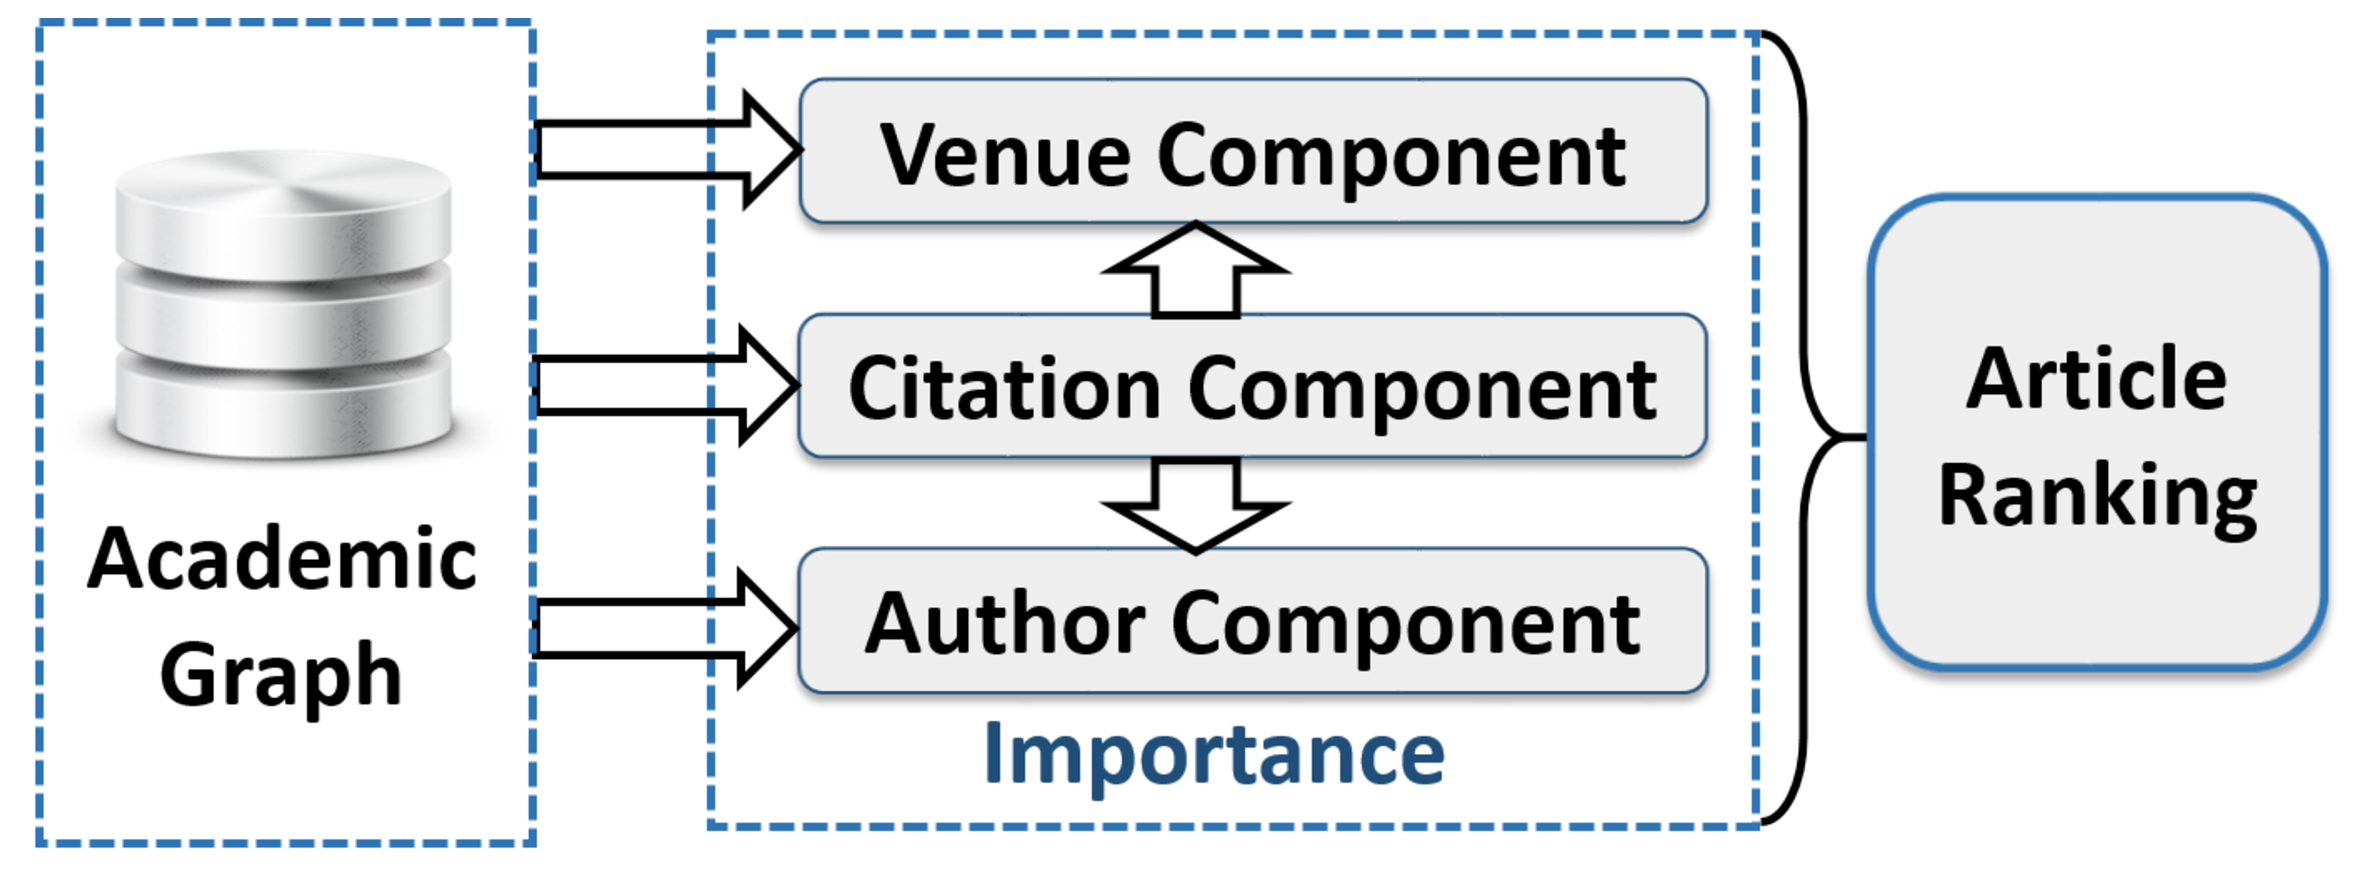
\includegraphics[scale=0.15]{framework-lite-2.eps}
%\vspace{-1ex}
\caption{\sarank framework~\cite{ma2018query}} \label{fig:sarank}
\vspace{-2ex}
\end{figure}
}%%%%%%%%%%EAT





\stitle{Citation counts and publish time}. Scholarly articles are simply sorted based on their citation counts and publish time. %, respectively, and ties are broken by further comparing importance scores.


\stitle{Importance}. This metric comes from our recently developed \sarank (please refer to~\cite{ma2018query} for details). The importance of an article is defined as a combination of its prestige and popularity, where its prestige is computed by a novel Time-Weighted PageRank, and its popularity is the sum of citation freshness. To assign those newly published articles reasonable ranking scores, it further assembles the importance of citations, authors and venues to derive the final ranking. %, as illustrated in Fig.~\ref{fig:sarank}.

The above three metrics are for {\em query independent ranking}, and we introduce two metrics for {\em query dependent ranking}.

\stitle{Relevance}. This metric enables to rank scholarly articles in terms of the semantic correlation between their titles and given queries (keywords). As Word2vec \cite{corrado2013efficient} has become the {\em de facto} standard to capture semantics, we utilize Word2vec to evaluate semantic relevance as follows.

%\begin{equation}
%\label{eq:relscore}
%rel(a, Q) = \sum_{t \in a.T} \sum_{q \in Q} idf(q) \frac {\textbf{t} \cdot \textbf{q}} {|| \textbf{t} ||\ ||\textbf{q}||}.
%\end{equation}

\marked{
\begin{equation}
\label{eq:relscore}
rel(a, Q) = \sum_{t \in a.T} \sum_{q \in Q} \frac {\textbf{t} \cdot \textbf{q}} {|| \textbf{t} ||\ ||\textbf{q}||}.
\end{equation}
}
\marked{
Here $a.T$ and $Q$ are the sets of words (excluding stop words) in the title of an article $a$ and the query, respectively, %$idf(q)$ is the inverse document frequency of a word $q$,
and $\textbf{t}$ and $\textbf{q}$ are their corresponding word embeddings. Although the entire article to compute the relevance can improves relevance accuracy, it is not the main concern of our work, we just briefly touch on this and will explore it in future work.}

% Reviewer 2
% Moreover, they say that the similarity to be captured is only between the query keywords and the article title, but do not explain why the entire text is not used.
% remove idf. I think idf(q) has no obvious effect. The reason is that we do not have the entire text.



\stitle{Relevant importance.} The previous importance metric does not consider the closeness of the articles with respect to given queries (keywords). This metric is to rank scholarly articles by combining the semantic relevance and importance metrics. More specifically, we first normalize the computed relevance (resp. importance) score by scaling with the maximum relevance (resp. importance) score in the resulting article set, and we then define the relevant importance score as follows.
\begin{equation}
\label{eq:relimp}
rImp(a, Q) = \alpha \cdot rel_n(a, Q) + (1-\alpha)\cdot imp_n(a),
\end{equation}
where $rel_n(a, Q)$ and $imp_n(a)$ are the {\em normalized} semantic relevance and importance scores, and $\alpha$ is a regularization parameter, typically set to an empirical value in $[0.2, 0.4]$.



\subsection{Author, Venue and Affiliation Ranking}
\label{subsec:heteroRanking}

For authors, venues and affiliations,  \oursystem provides stand-alone ranking and article-coupled ranking.

\stitle{Stand-alone ranking}. To support author, venue and affiliation searches, \oursystem ranks authors, venues and affiliations with the sum of the query independent ranking scores of all their associated articles. Further, when sorting entities by publish time, it uses an exponentially decayed ranking score $e^{T_a-T_0}$ to evaluate the research activeness of an entity, where $T_a$ is the publish year of an article $a$, and $T_0$ is the current year.

\stitle{Article-coupled ranking}. To support article search, \oursystem ranks authors, venues, and affiliations with respect to the resulting articles of an article search query, along the same lines as stand-alone ranking. This helps to answer questions like which authors (venues or affiliations) are the most authoritative ones in the query related field of study.


The search and ranking functions of \oursystem and existing systems are summarized in Table~I, where metrics are not reported due to their unavailability in commercial systems.



\eat{
-------------------- original version --------------------  \\
We first introduce Time-Weighted PageRank for evaluating the importance of entities, defined as a combination of the prestige and popularity, and then introduce entity ranking including author ranking, venue ranking, affiliation ranking and type ranking \itshape e.g., \upshape relevance ranking.


\subsection{Time-Weighted PageRank}
\par
PageRank is a typical method in scholarly articles ranking as we can easily make use of the reference between different articles. Due to the following reasons: (1) Different articles typically have different impacts in practice, and there is a need to differentiate, while PageRank essentially assumes equal impacts (2) The semantics of citation relationships are time-dependent, which means that citations at different periods of time may reveal different information. We introduce Time-Weighted PageRank(TWPageRank) by extending a time decay factor because of the impact of an article decay with time after peak time.
% why time weight pagerank

\par
We present TWPageRank that evaluate the prestige of nodes in a directed graph, in which each node attached with time information. And we use \itshape the impact weight \upshape to describe the relative weight from the edge sources to targets. Formally, the impact weight on a directed edge $(u,v), i.e.,$ an edge $u$ from $v$, is defined as:

\begin{equation}
\centering
\label{eq:edgeWeight}
w(u,v)=\left \{
\begin{array}{ccl}
1                        &    &{T_u   <   Peak_v} \\
e^{\sigma (T_u-Peak_v)}  &    &{T_u   \ge Peak_v} \\
\end{array} \right.
\end {equation}
where $T_u$ is the time of node $u$, $Peak_v$ is the peak time of node $v$ after which the impact weights of edges to $v$ decay with time, and $\sigma$ is a negative number controlling the decaying speed of the impacts. By default, we use years as its time granularity in Eq. (\ref{eq:edgeWeight}).

\par
Thus, the update rule of Time-weighted PageRank is

\begin{equation}
\centering
\label{eq:twPR}
PR(v)= d \sum_{(u,v)\in E} \frac{w(u,v)PR(u)}{W(u)} + \frac{1-d}{n}
\end{equation}
where $PR(u)$ and $PR(v)$ are the TWPageRank score of $u$ and $v$. And $E$ is a set of edges, $W(u)=\sum_v w(u,v)$ is the sum of the impact weights on all edges from $u$, $n$ is the number of nodes and $d$ is a damping parameter in (0, 1).
% what's TWpagerank


\subsection{Entity Ranking and Type Ranking}
\par
Scholarly entities(\itshape e.g., \upshape affiliation, venue, author and article) ranking is a problem of assessing the importance of nodes in a heterogeneous network. The importance is a combination of \itshape prestige \upshape and \itshape popularity \upshape to capture the evolving nature of entities. The prestige of scholarly entities is derived by applying TWPageRank on the citation graph $G$, and each type of entity is assigned the corresponding TWPageRank score as its prestige score $Prs$.

\par
To learn about the popularity of different scholarly entities, we first introduce the popularity of an article. The popularity of an article $v$ is the sum of all its citation freshness, \itshape i.e., \upshape the closeness to the current year:
\begin{equation}
\centering
\label{eq:pop}
Pop (v) = \sum_{(u,v) \in E^c} e^{\sigma(T_0 - T_u)}
\end{equation}
Here, $T_0$ is the current year, $T_u$ is the largest year among all articles, $\sigma$ is the negative decaying factor in Eq. (\ref{eq:edgeWeight}).

\par
Intuitively, prestige favors those with many citations soon after the publication of articles or associated articles of venues and authors, and popularity capture the temporal nature of entities.


\textbf{Affiliation Ranking.} We computes the importance of affiliations by their associated articles. As the importance of an affiliation evolves with time, we treat the affiliation importance in each year individually, and its importance is the sum of importance in all individual years.

\par
We construct an affiliation graph $G^a(V^a, E^a)$ using the citation information among affiliations, in which a node represents an affiliation in a specific year and a direct edge $(s, t)$  means that there exists articles of affiliation $s$ citing articles of affiliation $t$. Thus, the impact weights are defined as sums of impact weights from affiliation $s$ to affiliation $t$, \itshape i.e., \upshape
\begin{equation}
\centering
\label{eq:authorSumWeight}
w_a(s,t) = \sum_{u \in C(s), v \in C(t)} w(u,v)
\end{equation}
Here, $C(s)$ and $C(t)$ are the sets of articles of affiliation $s$ and affiliation $t$, and $w(u,v)$ is the impact weight of articles $u$ and $v$.
% define the impact weight between between author s and author t

\par
The prestige of an affiliation in a specific year ($Prs_a$) is computed using the impact weights Eq. (\ref{eq:authorSumWeight}) and the update rule in Eq. (\ref{eq:twPR}). The popularity of an affiliation in a specific year ($Pop_a$) is defined as the average popularity of its articles that is computed using Eq. (\ref{eq:pop}). Thus, the \itshape affiliation importance score \upshape ($Imp_a$) is defined as a combination of its prestige and popularity:
\begin{equation}
\centering
\label{eq:imp}
Imp_a(v) = Prs_a(v)^{\lambda} Pop_a(v)^{1-\lambda}
\end{equation}
Here, $\lambda \in [0, 1]$ is the importance factor, indicates the weighting about prestige and popularity.

\textbf{Venue Ranking.}
We computes the importance of venue using their associated articles which is similar with affiliation ranking. We treat the venue importance in each year, and construct a venue graph $G^v(V^v, E^v)$ using citation information among venues. And then we combine the prestige of a venue ($Prs_v$) and the popularity of venue ($Pop_v$) as the \itshape venue importance score \upshape ($Imp_v$).


\textbf{Author Ranking.}
We evaluate the importance of each author, and compute the average importance of the authors of an article as its \itshape author importance score. \upshape However, it is obvious that the author citation graph is too large to handle. Hence, we evaluate the prestige, popularity of the author by using the average prestige, popularity of all her/his published articles, respectively. Then, the author importance score ($Imp_{aut}$) is the combination of its prestige and popularity, similar to affiliation ranking.


\textbf{Article Ranking.}
If we are only to rank scholarly articles, the other type of entities such as venues and authors are closely involved. Hence, we assemble the importance of article, venue and author to produce the final scholarly articles ranking, illustrated in Fig. 1. Venue ranking and author ranking have presented in previous paragraphs. Next, introduce how to compute the importance of article using citation information.

\par
We first construct a citation graph $G^c(V^c, E^c)$ using citation information among articles. The prestige of articles ($Prs_c$) is derived by using TWPageRank in citation graph $G^c$. The popularity of an article ($Pop_c$)is the sum of all its freshness which has described in Eq. (\ref{eq:pop}). The importance of citation component ($Imp_c$) is a combination of its prestige and popularity in the citation graph by applying Eq. (\ref{eq:imp}).

\par
Thus, the static ranking score of an article $v$ is aggregated as follows:
\begin{equation}
\centering
\label{eq:assemble}
S(v) = \alpha Imp_v(v) + \beta Imp_{aut}(v) + (1 - \alpha - \beta)Imp_c(v)
\end{equation}
Here parameter $\alpha$, $\beta$ and $1- \alpha - \beta$  regularize the contributions of the venue, author and citation information.


\textbf{Relevance Ranking.} We have introduced affiliation, venue, author, article ranking in the former sections. These rankings are query independent and
aim to give a static ranking based on scholarly data only. However, it is vital to evaluate the similarity between the short query and sentence (\itshape i.e., \upshape title of the paper) when retrieve articles by keywords.

\par
Hence, we employ distributional semantic approach to represent words. Similarities between the term vectors indicates the corresponding semantic similarities \cite{corrado2013efficient}. The final ranking score of an article $v$ that relates to semantics of article title, defined as follow:
\begin{equation}
\centering
\label{eq:simscore}
F(v) = \theta S(v) + (1- \theta) \sum_j idf(Q_j) \frac {Q_j \cdot T} {\left \| Q_j \right \| \left \| T \right \|}
\end{equation}
Here, $S(v)$ is a static ranking score of article, $Q(j)$ is the j$th$ of query keywords vector which have removed stop words, $idf(Q_j)$ is inverse document frequency measures how much information the word $Q(j)$ provides, $T$ suggests we aggregate the title word vectors to their centroid and $\theta$ means the relevance factor.
} %%% end of \eat

\section{System Overview}
%\section{System Framework}
\label{sec-system}

\begin{figure}
\centering
\subfigure[{\scriptsize Framework}]{\label{fig:framework}
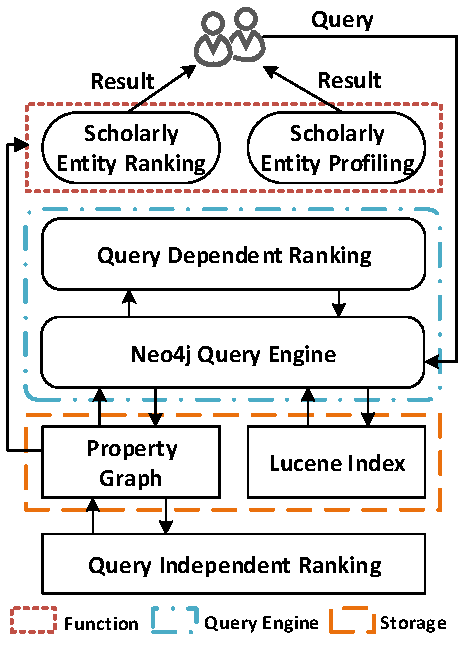
\includegraphics[width=0.4\columnwidth]{systemFrame.pdf}}
%\hspace{3ex}
\subfigure[{\scriptsize Neo4j schema}]{\label{fig:schema}
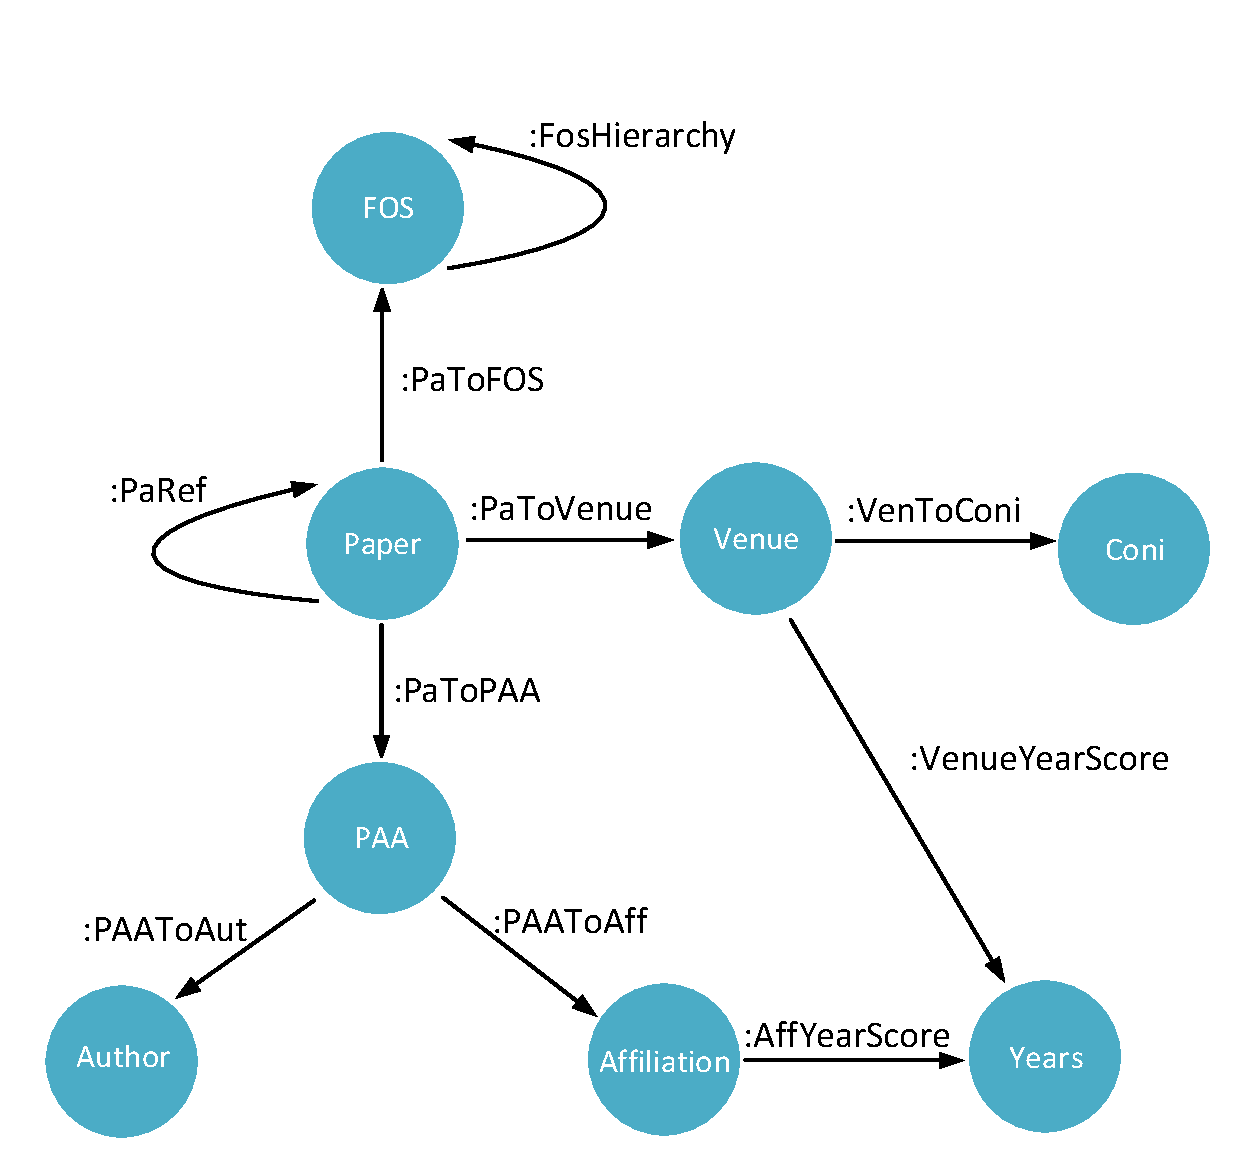
\includegraphics[width=0.56\columnwidth]{neo4jSchema.pdf}}
\caption{System design of \oursystem}
\label{fig:system}
%\vspace{-2ex}
\end{figure}


Figure \ref{fig:framework} shows the framework of our \oursystem. It consists of two main components, \ie \emph{Storage} and \emph{Query Engine}.
Below the storage component is a {\em Query-Independent Ranking} module that enriches the data with those pre-computed query-independent ranking scores. Note that there is another {\em Query-Dependent Ranking} module inside the query engine. Finally, two function modules on top present our analysis  to users based on the retrieved results. We next detail our system.

\subsection{Schema Design} \label{subsec:schema}

Graph database Neo4j is adopted for storage. As such, we need to design a schema that abstracts the entities and linked structures (\eg citation, authored-by).
% schema design rationaile
We follow two principles for schema design: (a) nodes for entities and relationships for linked structures, and (b) trading space for query efficiency if affordable and possible.

%reducing fine-grained relationship names while increase generic relationships qualified with property appropriately.

The schema is presented in Fig.~\ref{fig:schema}, where texts nears nodes and relationships represent properties of entities and linked structures, respectively.
It contains seven basic types of nodes including {\em Paper}, {\em Author}, {\em Affiliation}, {\em Venue}, {\em FOS} (field of study), {\em ConIns} (instances of conferences in each year) and {\em Year}.
In addition, it further incorporates an artificial type of nodes, \ie {\em PAA} representing paper-author-affiliation tuples. We use extra space to improve query efficiency, \ie an author and her/his affiliation can be retrieved in one query.
Our schema also forms a total of nine types of relationships, one of which, \ie {\em :VenueScore}, has a property {\em score} and the rest are unweighted.
As another space-efficiency trade-off, those {\em Paper} nodes also use extra space on properties to maintain conference ID, journal ID and year.



\subsection{Graph Storage} \label{subsec:storage}

%Thus, we model scholarly data as a huge heterogeneous graph, shown in Fig. \ref{fig:schema}, which contains more than one billion nodes and over two billion relationships.
% 126909021 paper  114698044 articles 529 million, node:1032827519, relationship:1933421586

Based on the above schema, we store our scholarly data, \ie MAG~\cite{sinha2015overview}, as a huge property graph with more than 1.03 billion nodes and over 1.93 billion relationships. We further clarify our graph storage with the following two points.

%Neo4j with native graph storage ensures that scholarly data is stored efficiently and relationships close to each other. We have proved through experiments that index-free adjacency is more efficient and cheaper, shown in Section~\ref{sec-demo}. Moreover, we highlight our graph storage on the following two points.
% neo4j native graph storage.

First, based on the original scholarly data, the {\em Query-Independent Ranking} module pre-computes those query-independent ranking metrics, \ie numbers of citations of papers, importance scores of papers, authors, venues and affiliations~\cite{ma2018query}. These scores are assigned as properties to the corresponding nodes.  As the most essential operation in the pre-computation, iteratively accessing the linked entities is much more convenient with graph storage.
Moreover, both citation numbers and importance scores support incremental computation~\cite{ma2018query} and are easier to dynamically maintain once the scholarly data get updated.

%given that our query independent ranking, a type of Time-Weighted PageRank based on graph, assesses the importance of nodes in the heterogeneous scholarly graph. Thus, it is much more convenient to compute the importance score when employ graph storage. Secondly,
%we recompute the scholarly graph once scholarly data gets updated through incremental algorithm~\cite{ma2018query}. We can easily operate the affected areas of the scholarly graph on the graph storage. (weak? we do not implement in \oursystem) However, a huge volume index in RDBMS will cause significant performance bottleneck when update.
% benefits��PageRank algorithm. incremental computation. update index??? in neo4j and mysql. in stages

Second, we utilize Lucene index to deal with query processing on the billion-scale property graph. More specifically, we create fulltext indices for paper titles and affiliation names. These enable to find papers and affiliations whose titles/names contain a specific word efficiently. We also create schema indices for paper ID, author names and venue names for initial entity lookup.

%Other properties, such as {\em Author name} and {\em Paper ID}, are also created index for initial entity lookups.
% lucene index. Why we need lucene index. index what. result.
%  with IKAnalyzer to support Chinese

\eat{
\marked{highlight graph storage, query engine detail}

\marked{relation to ranking model, when to do ranking}

\marked{incremental computation}


(2) property graph (billion-scale) -- lucene index
%(1) adopt neo4j
%(2)

Storage is a key factor for the success of scholarly analysis systems, due to the large volume of scholarly data (\eg \oursystem mainly uses the MAG data with 126 and 529 million articles and citations, respectively~\cite{sinha2015overview}) and the complex entities and relationships.
%
Traditional RDBMS are used by CiteSeerx, AMiner and Semantic Scholar to manage scholarly data. On the other hand, Acemap and Microsoft Academic exploit distributed file systems.
%
We observe that entities in scholarly data are inherently linked. The existing storage solutions all ignore such linked feature, and may face challenges for efficient and high-concurrent query processing when the computing resources are limited. For instance, complex join operations in RDBMS will become the bottleneck when processing queries such as {\em finding all articles of someone's co-authors}.
%
To this end, we propose to utilize a popular graph database Neo4j to store and manage the large-scale, heterogeneous and linked scholarly data in \oursystem.
}

%Scholarly data highly connected by reference relationship between articles and constructs a huge heterogeneous graph.  Take RDBMS as an example, complex joins and self-joins will incur obviously performance bottleneck when the scholarly dataset becomes more inter-related. A comparison of the performance of querying the cited articles of an article using RDBMS(Mysql) and graph database(Neo4j) is given in table 1. Furthermore, our heterogeneous entities ranking algorithm, a type of Time-Weighted PageRank bases on graph structure, assesses the importance of nodes in a heterogeneous graph. Thus, it utilizes a popular graph database Neo4j to store and manage heterogeneous scholarly data.
% scholarly data source, currently solution, why graph database.

%Intuitively, a paper get published in a journal/conference by the author means new edges among paper, author and venue node. By employing ranking model as stated in section \ref{sec-model}, we derive affiliation, author, venue and article ranking score using incremental computation \cite{ma2018query}. And those score is described as a property in the graph schema.
% explain our schema



% design principles and schema.
% We take into consideration of the query ability of the graph schema and adopt specific time and space trade-offs. heterogeneous scholarly entity ranking ?

%In fact, we can apply any other ranking algorithms to rank scholarly entities in the graph schema.


\subsection{Graph Query Engine} \label{subsec:qe}

\oursystem supports a variety of common queries on the property graph. And the graph {\em Query Engine} is responsible for processing this set of queries. When users issue a query, \oursystem first translates it into a cypher. The cypher is then sent to the {\em Neo4j Query Engine}, which generates a query plan after proper parsing and semantic analysis.
The query plan will hit Lucene index for initial entity lookup or directly process on the property graph. And the results are returned to the {\em Query-Dependent Ranking} module for further ranking computation, \ie the relevance and relevant importance scores.
An example query process of finding the top scholarly articles on ``graph database"  ranked by relevant importance is shown in Fig.~\ref{fig:queryProcess}.

\begin{figure}
\centering
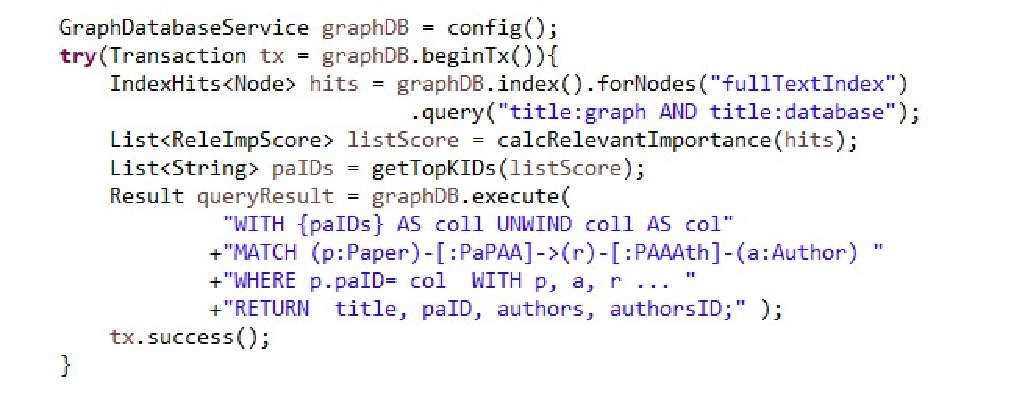
\includegraphics[width=\columnwidth]{queryProcess.pdf}
\caption{Query Process }
\label{fig:queryProcess}
\vspace{-3ex}
\end{figure}


%such as article retrieval, heterogeneous entity ranking and author topK fields of study��
%which consists of Query Dependent Ranking and Neo4j Query Engine.

% query dependent ranking
% Neo4j Query Engine
% cypher
% query engine detail, cypher execute, cypher example. take system function for example


%Generally speaking, heterogeneous entity query and heterogeneous entity profiling are supported by \oursystem. An example procedure is provided in Table~\ref{tab-codeExample}. We present how Query Engine works when retrieves Topk articles about keywords ``graph database" by {\em Relevant Importance} ranking metrics.
%cypher example. give an example.


%1. GraphDatabaseService graphDB = new GraphDatabaseFactory().. .newGraphDatabase(); \\
%2.    try(Transaction tx = graphDB.beginTx()){ \\
%3.		IndexHits<Node> hits = db.index().forNodes("fulltext") \\
%								.query("titile: graph AND title:database"); \\
%4.		List<ReleImpScore> listScore = calcRelevantImportance(hits); \\
%5.		List<String> paIDs = getTopKIDs(listScore); \\
%6.		Result result = graphDB.execute(" \\
%			WITH {paIDs} AS coll UNWIND coll AS col \\
%			MATCH (p:Paper)-[:PaPAA]->(r)-[:PAAAth]-(a:Author)\\
%			WHERE p.paID= col  WITH ... \\
%			RETURN  title, paID, authors, authorsID;\\
%		");	\\
%7.		tx.success();\\
%	}



\eat{
(1) ranking computation \& incremental
(2) functionality based on query engine
(3) example

\oursystem supports a variety of queries on scholarly data such as keyword retrieval, subgraph search, heterogeneous entity ranking. Query engine is the component responsible for processing a common set of queries on graph database. It consists of the Lucene index, query optimization, Neo4j query engine and ranking algorithms.
% add heterogenous entity Ranking ?

\oursystem takes advantage of Lucene inverted index and \marked{employs Lucene index in property of paper titles, author names and distributed representations of words.
%
Query optimization aims to reduce cardinality of work in the progress to generate a new query plan, such as hitting index, reducing matching paths. Moreover, Neo4j query engine executes the query plan to perform efficient data retrieval.
Finally, search results are aggregated by SARank, relevance, citation, year, average and maximum functions.}
}


\subsection{Visualization}

Finally, the two function modules on top collect the related scholarly entities and rankings returned from the back-end, and present some visual analysis to users. Moreover specifically, \oursystem utilizes RESTful APIs  and Echarts\footnote{http://echarts.baidu.com/} to display the scholarly ranking and profiling results. Detailed demonstrations are available in next section.


% visualization do what ?
% restful API
% scenarios, Query and Ranking Scholarly Entity, Author Profiling.
%Based on the graph storage, scholarly data was managed and processed in the system back-end. \oursystem collects user querys, dispatch to query engine and the results are then presented by visualizer using RESTful API. We employ Echarts (http://echarts.baidu.com/) to display scholarly article analysis and author profiling, detailed demonstrations are accessed in next section.
% function implement in back-end, echarts js  using RESTful API. demonstrate xxx in the next section.


%With scholarly data management and processing in the system back-end, the visualizer of \oursystem collects user queries through user interfaces. The queries are to the query engine and the returned results are then presented by visualizer. We will demonstrate some scholarly analysis scenarios in the next Section.


%\begin{table}[t!]
%%\begin{center}
%\caption{Query TopK Articles by Relevant Importance }
%\label{tab-codeExample}
%\begin{scriptsize}
%\begin{tabular}{ l}
%\hline
%{An Example procedure of Query TopK Articles by Relevant Importance } \\
%\hline
%1. GraphDatabaseService graphDB = new GraphDatabaseFactory()... ; \\
%2.  \hspace{6ex}  try(Transaction tx = graphDB.beginTx()) \{ \\
%3.  \hspace{12ex} 	IndexHits $\langle$ Node$\rangle$ hits = db.index().forNodes("fulltext") \\
%    \hspace{20ex}   .query("titile: graph AND title:database"); \\
%4.  \hspace{12ex} 	List$\langle$ ReleImpScore$\rangle$ listScore = calcRelevantImportance(hits); \\
%5.  \hspace{12ex} 	List$\langle$ String$\rangle$  paIDs = getTopKIDs(listScore); \\
%6.  \hspace{12ex}    Result result = graphDB.execute(`` \\
%    \hspace{20ex}		WITH \{paIDs\} AS coll UNWIND coll AS col \\
%    \hspace{20ex}		MATCH (p:Paper)-[:PaToPAA]-$>$(r)-[:PAAToAut]-(a:Author)\\
%	\hspace{20ex}		WHERE p.paID= col  WITH p, r, a, ... \\
%	\hspace{20ex}		RETURN  title, paID, authors, authorsID; ");\\
%7.	\hspace{12ex}	tx.success();\\
%    \hspace{6ex}  \} \\
%\hline
%\end{tabular} \\ %\vspace{.5ex}
%\end{scriptsize}
%%\end{center}
%\end{table}


\section{System Demonstration}\label{sec-demo}
\eat{
Storage is another key factor for the success of scholarly analysis systems, due to the large volume (\eg the MAG data contains 126 and 529 million articles and citations, respectively~\cite{sinha2015overview}) and the complex relationships between heterogeneous entities.
%Traditional RDBMS are used by CiteSeerx, AMiner and Semantic Scholar to manage scholarly data. On the other hand, Acemap and Microsoft Academic exploit distributed file systems.
Existing systems have exploited RDBMS or distributed file systems as the storage solutions.

Central to Athena is its ranking model that supports het-erogeneous scholarly entity ranking using various rankingmetrics.

% 1.query(various entity) and profiling (including ranking and the authority acja)2.author profiling , 3.efficiency MySQL and Neo4j. 
% We have built an online service for \oursystem. The functions are summarized in Table 1. We demonstrate two use cases in scholarly entity ranking and profiling. We also demonstrate the advantage of storage with Neo4j compared with RDBMS.

we demonstrate its ranking models and heterogenous entity rankings given the query keywords by \oursystem. (2) To further illustrate the effective ranking model based on importance, we take {\em time ranking} in SIGMOD as an example. (3) We also demonstrate author profiling for better knowledge of the author.

 Fig. \ref{fig: search keywords} is an example of Search Page. In this page, we fulfill the query need with their ranking metrics and
 construct keywords profiling, try to answer which authors/venues/affiliations are the most authoritative in the queried field of study.

}

\par The demonstration consists of three parts. (1) We walk through its various ranking metrics to demonstrate \oursystem on querying and heterogeneous entities ranking. (2) To further illustrate the profiling function based on scholarly data analysis, we take author profiling as an example. (3) The advantage of storage with Neo4j compared with RDBMS is demonstrated by experiment.
% heterogeneous entities ranking, ranking metrics 
% author profiling 
% storage advantage


\stitle{Querying and Ranking Scholarly Entity }. We demonstrate how to query and employ different ranking metrics to rank articles, as shown in \ref{fig: search keywords}. And heterogenous scholarly entities ranking is demonstrated for deep scholarly data analysis.

\par 
\oursystem is equipped with both searching articles and querying other academic entities, such as author, affiliation, journal, conference series and conference instance. Consider a query ``graph database". 

\stitle{Author profiling}. Fig. \ref{fig:hjwProfile} is an example of an Author Page, where contains author's basic information and author's detailed profiling. For basic information, users can check author's publications, related authors and author's affiliations. We also develop author's detailed profiling to have a knowledge of the author both from breadth and depth. Thus, we model the evolution of author's research interest, author's avatar with word cloud description, the statistics of publication, {\em etc}.

\stitle{Neo4j Compare with MySQL}


\begin{table}[t!]
\label{tab-function}
\begin{center}
\caption{Query efficiency Neo4j compared with rdbms}
\begin{scriptsize}
\begin{tabular}{ c c c c}
\hline
{} & {Paper Info} & {Author's TopK Papers} & {TopK Cited Articles' Info}\\ 
\hline 
MySQL & 0.251 s  & 6.493 s & 35.190 s \\
Neo4j & 0.239 s  & 3.062 s & 24.332 s \\
\hline

\end{tabular} \\ %\vspace{.5ex}
\end{scriptsize}
\end{center}
\end{table}

\eat{
\par
We equip \oursystem with both article retrieval and other academic entity retrieval, such as author, affiliations, journal, conference series and conference instance. We present influential papers about the keywords and {\em importance} for default ranking metric. In order to fit various ranking scenarios, \oursystem supports different ranking metrics such as {\em relevance}, {\em importance}, {\em citation}, {\em year}. {\em Relevance} is more suitable for retrieving articles by keywords, because of capturing semantic information. While {\em importance} is more appropriate for ranking articles of affiliation and venue. We also demonstrate top-k prestige authors, influential affiliations, famous journals/conferences corresponding to ranking metrics and keywords.

It has four major areas: (1) Area 1, the top of the picture, where users can search keywords, authors, affiliations, journal and conference (2) Area 2 presents influential papers about the keywords and {\em relevance} for default ranking metric, which is in the center of the picture. (3) At left of the picture is Area 3, users can specify different ranking metrics such as {\em relevance}, {\em importance}, {\em citation}, {\em year} to fit various ranking scenarios. (4) Top-k prestige authors, influential affiliations, famous journals/conferences corresponding to ranking metrics and keywords are shown in Area 4, which is at the right of the picture.
% keywords search and profiling.

\stitle{Ranking Instance} We rank the conference papers \eg SIGMOD following the metrics of {\em time ranking}. We only collect articles published earlier than 2016, so the top of {\em time ranking} is the maximum importance score in 2015. As shown in fig. \ref{fig:sigmod}, we put ``Spark SQL: Relational Data Processing in Spark" in second place, which has the most citations(653) in SIGMOD 2015 up to now. More generally, in our top 10, there are 3 articles that has the most citation in SIGMOD 2015.
% the description in ICDE 2018

\par
Although they share the same venue component in the same year, the author of the article has higher prestige and popularity, such as Matei Zaharia and Michael Armbrust. Besides, an article in VLDB cites the paper published in the same years that increases the prestige and popularity of the citation components. Thus, the paper possesses a higher importance score by assembling the component of citation, author and venue.
}


%\par
%\stitle{Affiliation profiling}. As shown in fig. \ref{}, we give an example of affiliation profiling. The layout of the Affiliation Page is similar with Search Page, users can discover publications using various ranking metrics and check statistics information, such as the importance author, relevant affiliation, famous journals/conferences.
%% affiliation profiling

%\par
%\stitle{Venue profiling} venue

\section{Conclusions}
\label{sec-conc}

In this paper, we have designed, developed and demonstrated a novel scholarly search system \oursystem to  facilitate the research activities of
scholars. \oursystem has supported rankings of four types of scholarly entities with five metrics, and provided profiling functions to enhance the understanding of scholarly data. Further, \oursystem has adopted a popular graph database Neo4j as the storage solution for efficient query processing on  billion-scale scholarly data.

%We exploit a popular graph database Neo4j as our storage solution to efficiently manage large volume scholarly data. Based on this, And \oursystem implements five ranking metrics to fit various ranking scenarios. In addition to rankings, we also implement heterogeneous entity profiling that presents some visual analysis for understanding scholarly broadly and deeply.


%In this paper, we design and develop a novel ranking system \oursystem to support heterogenous scholarly entity ranking including article, author, affiliation and venue rankings. And we employ a popular graph database Neo4j which is more efficient than RDBMS by experiment.
%\oursystem is equipped with five ranking metrics, namely {\em relevance}, {\em importance}, {\em relevant importance}, {\em citation} and {\em time}.


%In this paper, we design and develop a novel ranking system \oursystem to support heterogenous scholarly entity ranking including article, author, affiliation and venue rankings. In order fit the various ranking scenarios, our system is equipped with four ranking metrics, namely relevance, importance, citation and time. Moreover, by combining with different entities profiling, \oursystem help users have a better knowledge of the academic information both from breadth and depth. Thus, we gave an answer about the question which entities are the most authoritative in the queried field of study.



%In this paper, we present a novel ranking system for scholarly data, which aims to process the big scholarly data, rank heterogenous entities and analyse scholarly data to help researchers retrieve influential and recent works to inspire their future works. We develop Time-Weighted PageRank for evaluating the importance of entities and assemble the article, venue and author for scholarly article ranking. Moreover, we construct a huge heterogenous academic data property graph based on its structure to manage and operate scholarly data efficiently. We have also designed visualization in the system to provide better service for researchers





% trigger a \newpage just before the given reference
% number - used to balance the columns on the last page
% adjust value as needed - may need to be readjusted if
% the document is modified later
%\IEEEtriggeratref{8}
% The "triggered" command can be changed if desired:
%\IEEEtriggercmd{\enlargethispage{-5in}}

% references section

% can use a bibliography generated by BibTeX as a .bbl file
% BibTeX documentation can be easily obtained at:
% http://mirror.ctan.org/biblio/bibtex/contrib/doc/
% The IEEEtran BibTeX style support page is at:
% http://www.michaelshell.org/tex/ieeetran/bibtex/
%\bibliographystyle{IEEEtran}
% argument is your BibTeX string definitions and bibliography database(s)
%\bibliography{IEEEabrv,../bib/paper}
%
% <OR> manually copy in the resultant .bbl file
% set second argument of \begin to the number of references
% (used to reserve space for the reference number labels box)

% \begin{thebibliography}{1}

% \bibitem{IEEEhowto:kopka}
% H.~Kopka and P.~W. Daly, \emph{A Guide to \LaTeX}, 3rd~ed.\hskip 1em plus
%   0.5em minus 0.4em\relax Harlow, England: Addison-Wesley, 1999.

% \end{thebibliography}

\bibliographystyle{IEEEtran}
\bibliography{refs}

\end{document}


